\documentclass[aspectratio=169,11pt]{beamer}
\usepackage[T1]{fontenc}
\usepackage{lmodern}
\usepackage[spanish]{babel}
\usepackage{booktabs,array,tabularx}
\usepackage{tikz}
\usetikzlibrary{arrows.meta,positioning}
\definecolor{ink}{HTML}{111827}
\definecolor{muted}{HTML}{475569}
\definecolor{teal}{HTML}{087F72}
\definecolor{mist}{HTML}{E6F5F1}
\definecolor{warn}{HTML}{B45309}
\definecolor{bad}{HTML}{B91C1C}
\setbeamercolor{normal text}{fg=ink,bg=white}
\setbeamercolor{frametitle}{fg=ink}
\setbeamercolor{structure}{fg=teal}
\setbeamercolor{block title}{fg=white,bg=teal}
\setbeamercolor{block body}{bg=mist,fg=ink}
\setbeamerfont{frametitle}{series=\bfseries}
\setbeamertemplate{navigation symbols}{}
\setbeamertemplate{itemize items}{\color{teal}\textbullet}
\setbeamertemplate{footline}{\hspace{1em}\scriptsize\color{muted} OLIST LAB \textperiodcentered{} DS3031 \textperiodcentered{} Entrega final Tipo 2\hfill\insertframenumber/\inserttotalframenumber\hspace{1em}\vspace{.6em}}
\newcommand{\kpi}[2]{\begin{minipage}[t]{.23\textwidth}\color{teal}\LARGE\bfseries #1\par\scriptsize\normalfont\color{muted}#2\end{minipage}}
\newcommand{\ok}{\textcolor{teal}{\textbf{\checkmark}}}
\newcolumntype{Y}{>{\raggedright\arraybackslash}X}
\tikzset{olistbox/.style={draw=teal,fill=mist,rounded corners=5pt,align=center,minimum height=1.0cm,text width=2.3cm,font=\scriptsize},flow/.style={-{Stealth},thick,draw=teal}}
\begin{document}

% 1 ------------------------------------------------------------------------------------------
{
\setbeamercolor{normal text}{fg=white,bg=ink}
\begin{frame}[plain]
\color{white}
\small DS3031 \textperiodcentered{} ÉTICA Y SEGURIDAD DE DATOS \textperiodcentered{} PROYECTO FINAL TIPO 2
\vfill
{\fontsize{35}{40}\selectfont\bfseries Olist Lab\par}
\medskip
{\Large Panel seguro de entregas: analizar sin exponer personas\par}
\vfill
\small Ronal Jesús Condor Blas \quad / \quad Marco Soto Maceda\\[2pt]
\scriptsize\color{white!70!ink} github.com/ronaljcb/proyecto-etica-seguridad-olist \quad\textperiodcentered\quad ronaljcb.github.io/proyecto-etica-seguridad-olist
\end{frame}
}

% 2 ------------------------------------------------------------------------------------------
\begin{frame}{¿Dónde investigar las demoras sin exponer clientes?}
\kpi{96\,470}{pedidos entregados analizados}\hfill
\kpi{6.8\,\%}{llegaron tarde (6\,534)}\hfill
\kpi{10.6 d}{retraso medio de los tardíos}\hfill
\kpi{4.29\,/\,2.27}{reseña puntual / tardía}
\bigskip
\begin{columns}[T,onlytextwidth]
\column{.5\textwidth}
\small\textbf{Riesgo:} el dataset original enlaza clientes, vendedores, ciudades, pagos y texto libre. Compartir filas para analizar expone a personas.
\column{.46\textwidth}
\small\textbf{Solución:} panel con \emph{solo agregados}, base cifrada, acceso con roles, HTTPS con CA propia y recuperación verificada.
\end{columns}
\vfill
\scriptsize\color{muted} Datos históricos 2016--2018 (Olist, Kaggle) + feriados de Brasil 2018. Comparaciones descriptivas, no causales.
\end{frame}

% 3 ------------------------------------------------------------------------------------------
\begin{frame}{Resumen: qué logramos en el avance y qué añade la entrega final}
\small
\begin{columns}[T,onlytextwidth]
\column{.47\textwidth}
\begin{block}{Avance (E1)}
\begin{itemize}\setlength\itemsep{1pt}
\item Importación mínima + panel React/Flask
\item SQLCipher en reposo, contraseñas con hash
\item Roles, CSRF, auditoría
\item Respaldo AES-256-GCM restaurable
\item HTTPS con certificado temporal
\item DPIA inicial y plan de incidentes
\end{itemize}
\end{block}
\column{.5\textwidth}
\begin{block}{Entrega final (EF)}
\begin{itemize}\setlength\itemsep{1pt}
\item \textbf{CA propia} y certificado TLS formal
\item \textbf{Herramientas}: Bandit, pip-audit, npm audit, gitleaks, CI
\item 35 pruebas + 20 comprobaciones en vivo
\item ZIP sellado, \texttt{seller\_id} retirado
\item Supresión $k{=}30$ \emph{en el servidor} + complementaria
\item Revocación de sesiones, bloqueo por IP, retención
\item Respuesta a un \textbf{incidente real}
\end{itemize}
\end{block}
\end{columns}
\end{frame}

% 4 ------------------------------------------------------------------------------------------
\begin{frame}{Arquitectura}
\centering
\begin{tikzpicture}[node distance=7mm,olistbox/.append style={text width=2.0cm}]
\node[olistbox] (zip) {ZIP Olist\\sellado AES-GCM};
\node[olistbox,right=of zip] (imp) {Importador\\solo 8 columnas};
\node[olistbox,right=of imp] (db) {SQLCipher\\AES-256 + HMAC};
\node[olistbox,right=of db] (api) {Flask API\\sesión, roles, $k{=}30$};
\node[olistbox,right=of api] (web) {React\\agregados};
\node[olistbox,below=9mm of db] (bk) {Respaldo\\AES-256-GCM, rotación};
\node[olistbox,below=9mm of api] (ca) {CA propia\\ECDSA P-384};
\node[olistbox,below=9mm of web] (log) {Auditoría\\retención 180 d};
\draw[flow] (zip)--(imp); \draw[flow] (imp)--(db); \draw[flow] (db)--(api);
\draw[flow,<->] (api)--node[above=2pt,font=\tiny]{TLS}(web);
\draw[flow] (db)--(bk); \draw[flow,dashed] (ca)--node[right,font=\tiny]{certificado}(api); \draw[flow] (api)--(log);
\end{tikzpicture}
\bigskip

\small Servidor solo en \texttt{127.0.0.1}. Claves separadas (\texttt{db}, \texttt{backup}, \texttt{source}) con permisos 0600 y carpeta configurable.
\end{frame}

% 5 ------------------------------------------------------------------------------------------
\begin{frame}{Cumplimiento: requerimientos funcionales}
\footnotesize
\begin{tabularx}{\textwidth}{@{}l Y c c@{}}
\toprule
ID & Requerimiento & Entrega & Estado\\
\midrule
F1 & Importar Olist + feriados y consultar agregados & E1 & \ok\\
F2 & KPIs, filtro por estado y serie mensual & E1 & \ok\\
F3 & Comparación feriado / día común con tamaños de grupo & E1 & \ok\\
F4 & Acceso con cuenta; auditoría solo para admin & E1 & \ok\\
F5 & Respaldo, restauración y contingencia (base, ZIP, código) & E1/EF & \ok\\
F6 & Administración de cuentas y purga de logs por consola & EF & \ok\\
F7 & Panel por HTTPS con certificado de la CA propia & EF & \ok\\
F8 & Registros individuales / análisis por vendedor & --- & \textcolor{warn}{descartado por la DPIA}\\
\bottomrule
\end{tabularx}
\medskip

\small El usuario usa \emph{su} información con el fin previsto: las medidas no bloquean el análisis, solo la exposición individual.
\end{frame}

% 6 ------------------------------------------------------------------------------------------
\begin{frame}{Cumplimiento: requerimientos de seguridad}
\scriptsize
\begin{tabularx}{\textwidth}{@{}l Y Y c@{}}
\toprule
ID & Requerimiento del curso & Cómo lo cumplimos & \\
\midrule
S01 & Encriptación en reposo & SQLCipher, ZIP sellado AES-GCM, claves 0600 separables & \ok\\
S02 & Transporte + certificados digitales & TLS $\geq$1.2 (1.3 en la prueba), CA propia, HSTS & \ok\\
S03 & Hashing & scrypt con sal, política de contraseñas & \ok\\
S04 & Gestión de accesos & Roles, CSRF, sesión 30 min revocable, bloqueo usuario/IP & \ok\\
S05 & Registros de auditoría & 12 tipos de evento, sin contraseñas, retención 180 d & \ok\\
S06 & Backups y recuperación & AES-GCM autenticado, rotación, \texttt{integrity\_check} & \ok\\
S07 & Herramienta de análisis & Bandit, pip-audit, npm audit, gitleaks, pytest, CI & \ok\\
S08 & Políticas, procedimientos, formación & Política de 7 reglas, ejercicio sobre incidente real & \ok\\
S09 & Riesgos y entidades afectadas & Modelo de amenazas + DPIA & \ok\\
S10 & Plan de incidentes y mejoras futuras & NIST SP 800-61 aplicado; 8 recomendaciones & \ok\\
\bottomrule
\end{tabularx}
\end{frame}

% 7 ------------------------------------------------------------------------------------------
\begin{frame}{Certificados digitales: de \emph{adhoc} a una CA propia}
\small
\begin{columns}[T,onlytextwidth]
\column{.52\textwidth}
\textbf{\texttt{pki.py}}
\begin{itemize}\setlength\itemsep{2pt}
\item \textbf{CA raíz}: ECDSA P-384, 5 años, \texttt{CA=true, pathlen=0}, clave PKCS\#8 cifrada
\item \textbf{Servidor}: ECDSA P-256, 397 días, SAN \texttt{localhost}, \texttt{127.0.0.1} y \texttt{::1}, \texttt{serverAuth}, \texttt{CA=false}
\item TLS mínimo 1.2 + HSTS
\end{itemize}
\column{.44\textwidth}
\begin{block}{Prueba automatizada}
\scriptsize Cliente con la CA: \textbf{TLS 1.3}, \texttt{AES\_256\_GCM\_SHA384}, cadena y host verificados.\\[3pt]
Cliente sin la CA: \textbf{conexión rechazada}.
\end{block}
\end{columns}
\medskip
\small La confianza pasa a ser una \textbf{decisión explícita} (instalar la raíz), no la costumbre de ignorar advertencias.
\end{frame}

% 8 ------------------------------------------------------------------------------------------
\begin{frame}{Accesos y auditoría}
\begin{columns}[c,onlytextwidth]
\column{.56\textwidth}
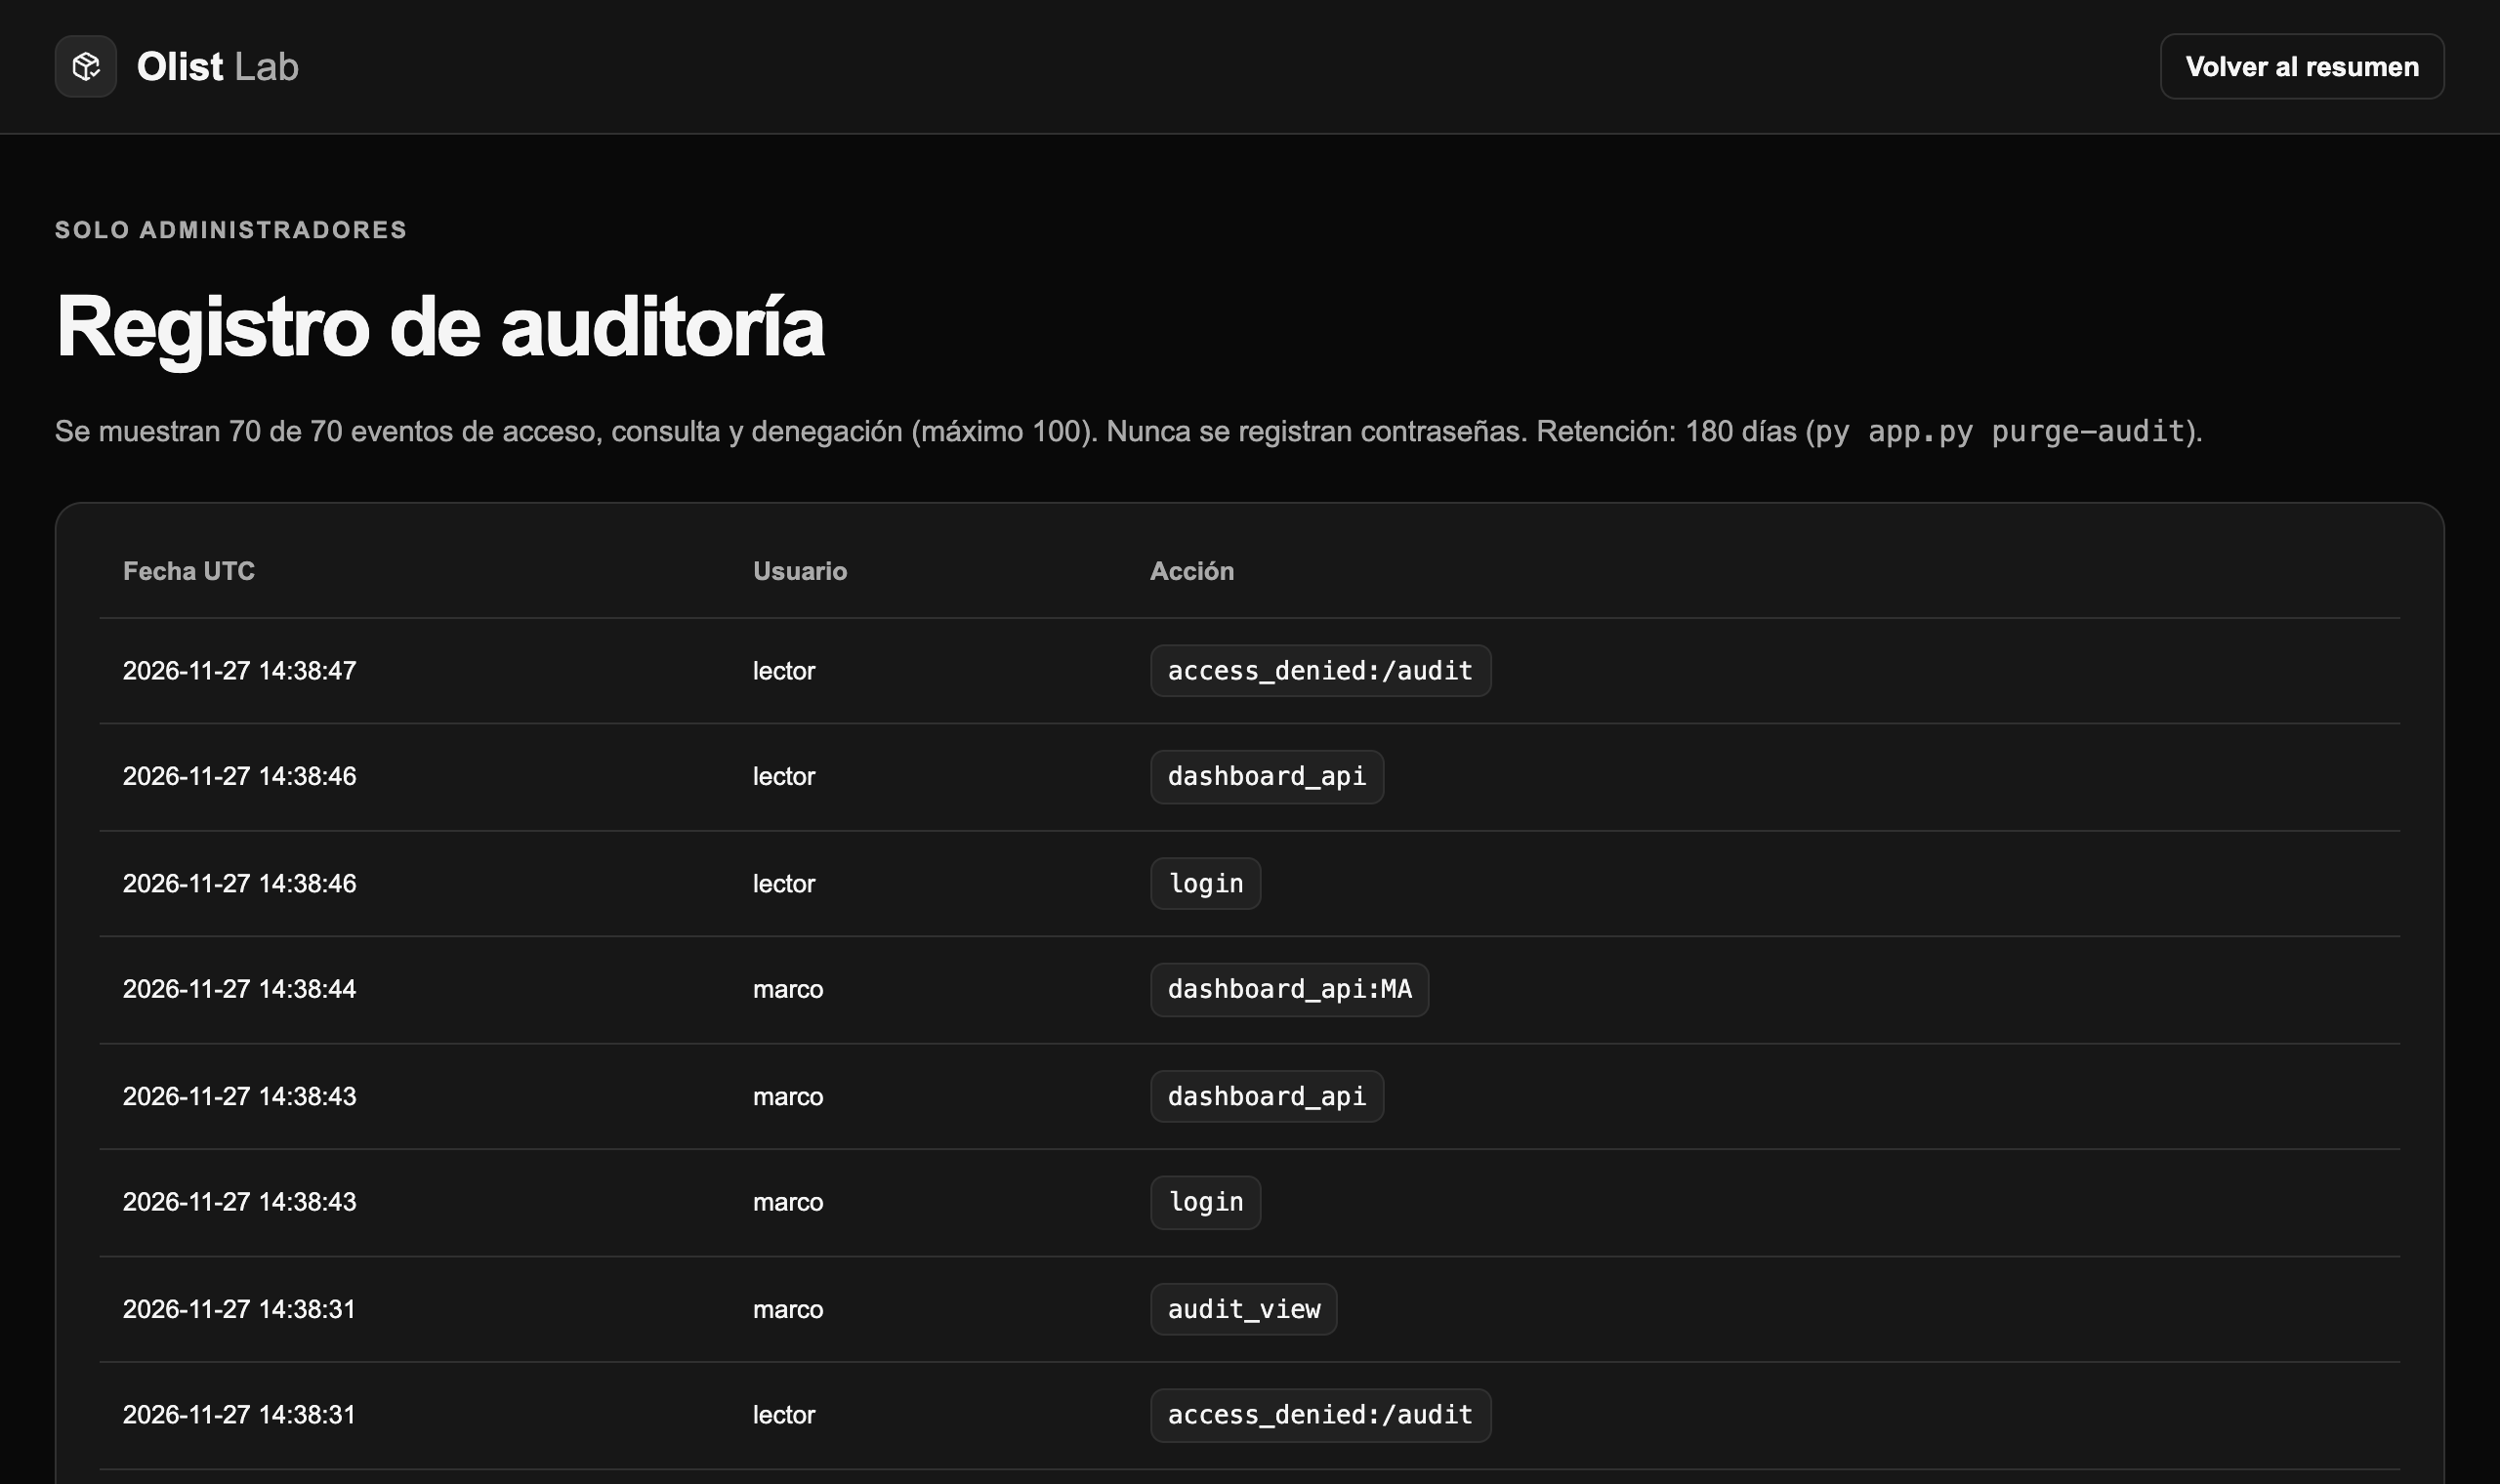
\includegraphics[width=\linewidth]{fig3_auditoria_rbac.png}
\column{.40\textwidth}
\small
\begin{itemize}\setlength\itemsep{2pt}
\item Lector en \texttt{/audit} $\Rightarrow$ \textbf{403} y evento \texttt{access\_denied}
\item 5 fallos/usuario o 20/IP en 15 min $\Rightarrow$ \textbf{429}
\item Cambiar clave o borrar cuenta \textbf{revoca} sesiones abiertas
\item Nunca se registran contraseñas
\end{itemize}
\end{columns}
\end{frame}

% 9 ------------------------------------------------------------------------------------------
\begin{frame}{Herramientas de análisis: hallazgos y correcciones}
\scriptsize
\begin{tabularx}{\textwidth}{@{}l l Y Y c@{}}
\toprule
Herramienta & Tipo & Hallazgo & Corrección & Final\\
\midrule
Bandit & SAST & \textcolor{bad}{4 B101}: \texttt{assert} validaba el certificado (se borra con \texttt{-O}); 3 B608 en E1 & Validación explícita; SQL fijo & \textbf{0}\\
npm audit & SCA & \textcolor{bad}{15 CVE (7 altas)}: \texttt{undici}, \texttt{hono}, \texttt{zod}\dots{} vía CLI \texttt{shadcn} & CLI a \texttt{devDependencies}; quitar \texttt{cn} & \textbf{0}\\
pip-audit & SCA & Sin vulnerabilidades & --- & \textbf{0}\\
gitleaks & Secretos & 0 alertas\dots{} pero había 2 contraseñas reales & Revisión manual + rotación & ---\\
pytest & Pruebas & S01--S06, P01, F1--F3 & --- & \textbf{35/35}\\
\bottomrule
\end{tabularx}
\medskip

\small\textbf{Lección:} el riesgo estaba en las dependencias, y ninguna herramienta reemplaza la revisión humana. CI en cada \emph{push} y cada lunes, con Dependabot.
\end{frame}

% 10 -----------------------------------------------------------------------------------------
\begin{frame}{Verificación en vivo sobre la instancia real: 20/20}
\centering
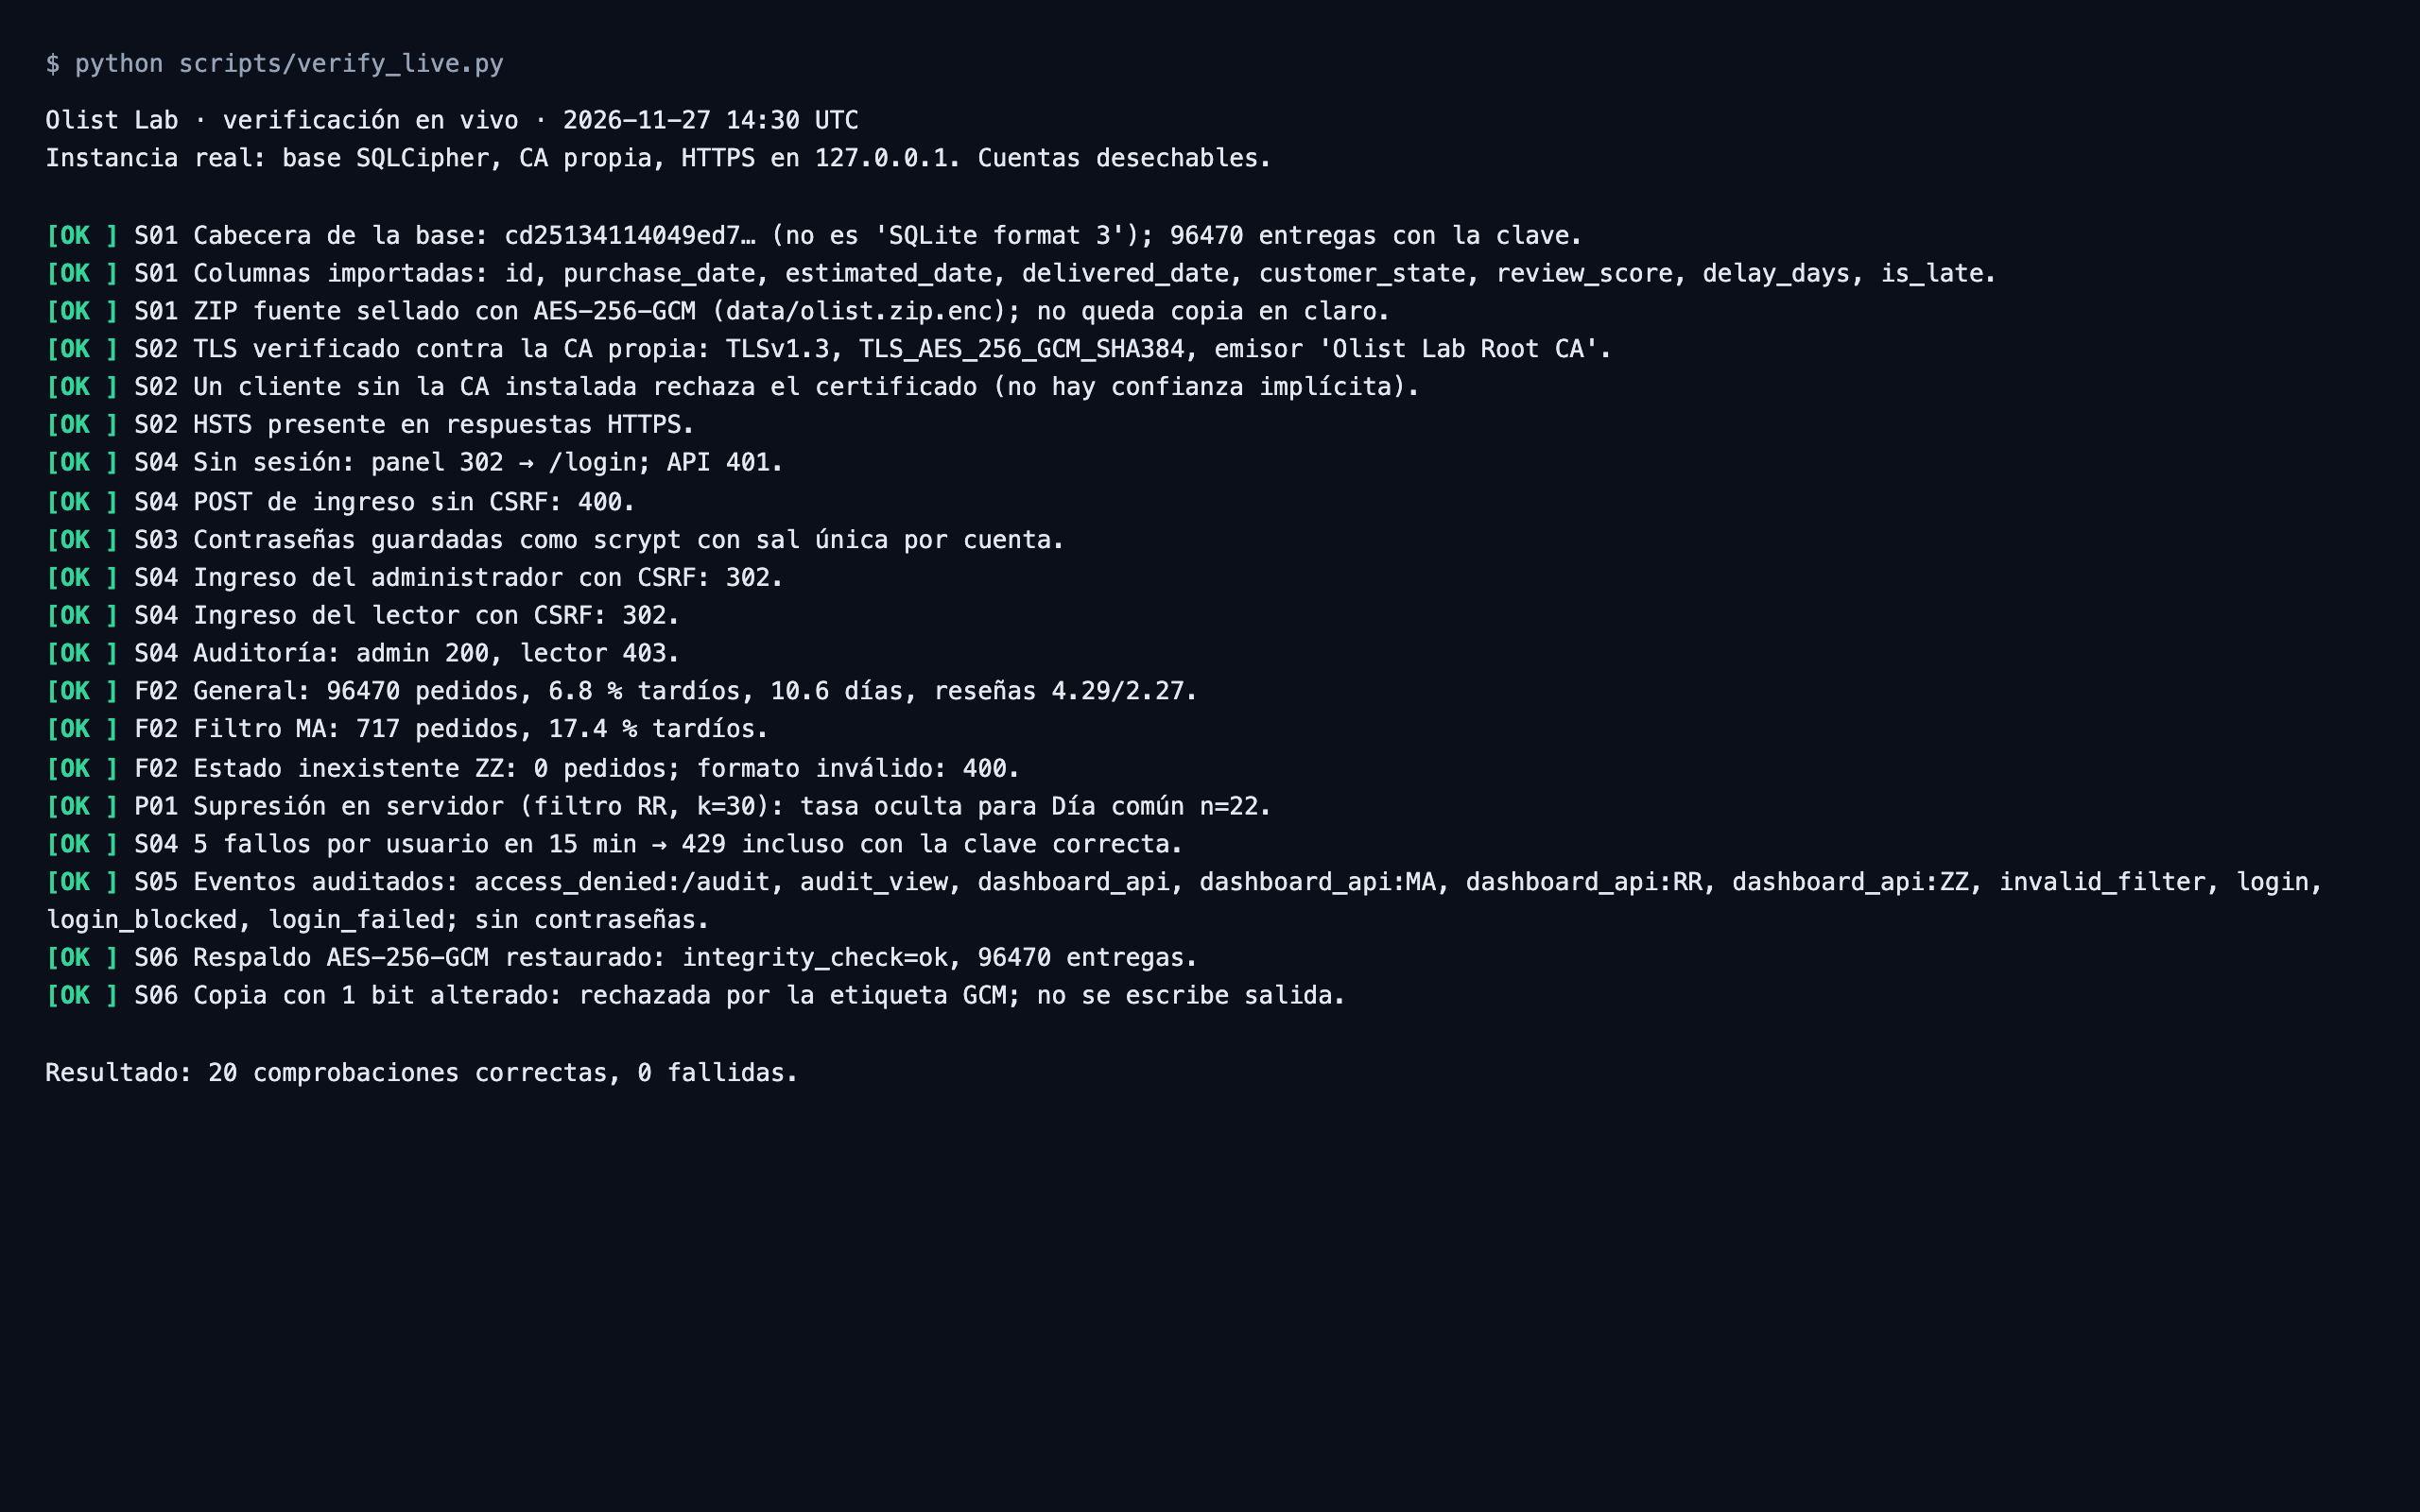
\includegraphics[height=.78\textheight]{fig4_seguridad_recuperacion.png}
\end{frame}

% 11 -----------------------------------------------------------------------------------------
\begin{frame}{Incidente real: credenciales de demo publicadas}
\centering
\begin{tikzpicture}[node distance=4mm]
\node[olistbox,text width=2.0cm] (a) {\textbf{Detección}\\revisión manual: 2 contraseñas en un script público};
\node[olistbox,text width=2.0cm,right=of a] (b) {\textbf{Análisis}\\cuentas solo locales; sin datos de clientes};
\node[olistbox,text width=2.0cm,right=of b] (c) {\textbf{Contención}\\rotación aleatoria + revocar sesiones};
\node[olistbox,text width=2.0cm,right=of c] (d) {\textbf{Recuperación}\\script lee el entorno; verificación 20/20};
\node[olistbox,text width=2.0cm,right=of d] (e) {\textbf{Mejora}\\gitleaks en CI, regla 3 de la política};
\draw[flow] (a)--(b); \draw[flow] (b)--(c); \draw[flow] (c)--(d); \draw[flow] (d)--(e);
\end{tikzpicture}
\bigskip

\small Plan basado en NIST SP 800-61 r3. \textbf{Borrar el archivo no borra el historial}: la mitigación real es rotar el secreto.\\
Lo usamos como ejercicio de \textbf{formación} del equipo.
\end{frame}

% 12 -----------------------------------------------------------------------------------------
\begin{frame}{Contingencia y recuperación}
\small
\begin{columns}[T,onlytextwidth]
\column{.5\textwidth}
\begin{itemize}\setlength\itemsep{3pt}
\item \textbf{Base}: \texttt{backup.py backup -{}-keep 7}
\item \textbf{Restauración} a otra ruta + \texttt{integrity\_check}
\item \textbf{ZIP}: sellado; si se pierde, se descarga y se verifica su SHA-256
\item \textbf{Código}: GitHub + espejo + clones; \texttt{git bundle}
\item \textbf{CA}: se reemite con \texttt{pki.py init}
\end{itemize}
\column{.46\textwidth}
\centering
\begin{tikzpicture}[node distance=5mm]
\node[olistbox] (a) {Base cifrada};
\node[olistbox,below=of a] (b) {Respaldo GCM};
\node[olistbox,below=of b] (c) {96\,470 filas, \texttt{ok}};
\draw[flow] (a)--(b); \draw[flow] (b)--(c);
\node[right=2mm of b,text width=2.6cm,font=\scriptsize,text=bad] {1 bit alterado $\Rightarrow$ rechazado, sin salida};
\end{tikzpicture}
\end{columns}
\end{frame}

% 13 -----------------------------------------------------------------------------------------
\begin{frame}{DPIA: riesgos, afectados y ética}
\scriptsize
\begin{tabularx}{\textwidth}{@{}p{3.1cm} p{2.3cm} Y c c@{}}
\toprule
Riesgo & Afectados & Control & Inicial & Residual\\
\midrule
Exposición de ZIP o claves & compradores, vendedores & ZIP sellado, SQLCipher, sin IDs & Alto & Medio-bajo\\
Reidentificación por grupos & compradores & $k{=}30$ en el servidor + complementaria & Alto & Bajo\\
Cuentas y trazas & equipo & scrypt, revocación, retención & Alto & Medio\\
Interpretación injusta & vendedores, regiones & denominadores, sin lenguaje causal & Medio & Bajo\\
Pérdida de datos & continuidad & respaldo verificado & Alto & Medio\\
\bottomrule
\end{tabularx}
\medskip

\small\textbf{Ética:} que el dataset sea público no implica consentimiento para cualquier uso. Las reseñas tienen \emph{sesgo de autoselección}. Las tasas regionales reflejan logística, no a las personas.\\
\textbf{Marco legal:} Ley 29733 y su reglamento (Perú), y LGPD (Brasil).
\end{frame}

% 14 -----------------------------------------------------------------------------------------
\begin{frame}{Uso seguro: política y formación}
\small
\begin{columns}[T,onlytextwidth]
\column{.55\textwidth}
\begin{enumerate}\setlength\itemsep{1pt}
\item Finalidad académica y agregada
\item Una cuenta por persona, mínimo privilegio
\item \textbf{Ningún secreto en el código}
\item No publicar ZIP, base, claves ni respaldos
\item CA solo en los equipos de la demo
\item Logs 180 días; borrado al cerrar el curso
\item Mostrar denominadores; no afirmar causas
\end{enumerate}
\column{.41\textwidth}
\begin{block}{Formación del equipo}
\scriptsize Ejercicio sobre el incidente real: reconocer el secreto, aplicar el plan, restaurar un respaldo y distinguir HTTP local de HTTPS validado.
\end{block}
\end{columns}
\end{frame}

% 15 -----------------------------------------------------------------------------------------
\begin{frame}{Recomendaciones futuras (no implementadas, justificadas)}
\small
\begin{columns}[T,onlytextwidth]
\column{.49\textwidth}
\begin{itemize}\setlength\itemsep{2pt}
\item \textbf{KMS/HSM}: claves fuera del equipo
\item \textbf{MFA} (TOTP o WebAuthn)
\item \textbf{WSGI + proxy + CA pública}
\item \textbf{Privacidad diferencial} (OpenDP) frente a consultas combinadas
\end{itemize}
\column{.49\textwidth}
\begin{itemize}\setlength\itemsep{2pt}
\item \textbf{SIEM} y logs de solo anexado
\item Respaldos \textbf{fuera del sitio} con RPO/RTO
\item Hook \textbf{pre-commit} con reglas propias
\item Roles \texttt{analyst}/\texttt{reader} diferenciados
\end{itemize}
\end{columns}
\end{frame}

% 16 -----------------------------------------------------------------------------------------
\begin{frame}{Lecciones aprendidas y retrospectiva}
\small
\begin{columns}[T,onlytextwidth]
\column{.49\textwidth}
\textbf{Lecciones}
\begin{itemize}\setlength\itemsep{1pt}
\item Definir el KPI antes de importar: ``por si acaso'' no es una finalidad
\item Ocultar en la interfaz no es un control
\item Las dependencias son la mayor superficie de ataque
\item Un respaldo se prueba restaurándolo
\end{itemize}
\column{.49\textwidth}
\textbf{Retrospectiva}
\begin{itemize}\setlength\itemsep{1pt}
\item[\textcolor{teal}{+}] La DPIA como lista de tareas; evidencia automatizada
\item[\textcolor{bad}{--}] Secretos en scripts; controles pensados primero en la interfaz
\item[\textcolor{teal}{$\rightarrow$}] CI y hooks desde el primer commit; una prueba por requerimiento
\end{itemize}
\end{columns}
\end{frame}

% 17 -----------------------------------------------------------------------------------------
\begin{frame}{Demostración en vivo (6--8 min)}
\small
\begin{enumerate}\setlength\itemsep{2pt}
\item \texttt{py pki.py show} y \texttt{py app.py run} $\rightarrow$ \texttt{https://127.0.0.1:5000} con candado (CA instalada)
\item Admin: KPIs 96\,470 $\rightarrow$ filtro MA (717) $\rightarrow$ Auditoría
\item Lector: \texttt{/audit} $\rightarrow$ 403, que queda registrado
\item \texttt{backup.py backup} / \texttt{restore}, y una copia alterada que se rechaza
\item \texttt{scripts/security\_scan.sh} y \texttt{scripts/verify\_live.py} $\rightarrow$ 0 hallazgos, 35/35, 20/20
\end{enumerate}
\vfill
\centering\large\textbf{Gracias} \quad\normalsize\color{muted} ¿Preguntas?
\end{frame}
\end{document}
